\documentclass[conference]{IEEEtran}
\IEEEoverridecommandlockouts
% The preceding line is only needed to identify funding in the first footnote. If that is unneeded, please comment it out.
\usepackage{cite}
\usepackage{amsmath,amssymb,amsfonts}
\usepackage{algorithmic}
\usepackage{graphicx}
\usepackage{textcomp}
\usepackage{xcolor}
\usepackage{enumerate}
\usepackage{booktabs}
\usepackage{float}
\usepackage{hyperref}
\usepackage{subfigure}
\usepackage{subcaption}
\usepackage{tabularx}
\def\BibTeX{{\rm B\kern-.05em{\sc i\kern-.025em b}\kern-.08em
    T\kern-.1667em\lower.7ex\hbox{E}\kern-.125emX}}
\begin{document}

\title{Group 6 Milestone 2: FracTrack\\[0.5em] 
       \large Deep Learning for X-Ray Fracture Analysis}
\author{Your Name}
\author{\IEEEauthorblockN{Srivatsa Balasubramanyam}
\IEEEauthorblockA{\textit{University of Virginia} \\
\textit{School of Data Science}\\
Parkland, Florida \\
mhe3sy@virginia.edu}
\and
\IEEEauthorblockN{Claire Sullivan}
\IEEEauthorblockA{\textit{University of Virginia} \\
\textit{School of Data Science}\\
Charlottesville, Virginia \\
kyq5rs@virginia.edu}
\and
\IEEEauthorblockN{Jasmine Waller}
\IEEEauthorblockA{\textit{University of Virginia} \\
\textit{School of Data Science}\\
Charlottesville, Virginia \\
vwx5pn@virginia.edu}
\and
\IEEEauthorblockN{Kristina Quintana}
\IEEEauthorblockA{\textit{University of Virginia} \\
\textit{School of Data Science}\\
Charlottesville, Virginia \\
kvq4nvn@virginia.edu}
}

\maketitle

\section{Abstract}
Progress has been made on both the development and implementation side of the use of AI in the medical field. Specifically, one area of growth has been the use of deep convolutional neural networks (CNNs) image architectures to assist in the processing of medical imaging. In this project, we develop a fine-tuned fracture detection model based on pre-trained ConvNeXT, designed to be used in the clinic as a first line of defense for detecting the need for medical care based on radiographic images. We implemented a multi-task classification model to identify upper extremity body parts and the presence of bone abnormalities. We show how the use of this model is an improvement over the well established ResNet-50 architecture. We explored methods including data augmentation and evaluated our model for cross-data generalization. Our code and pre-processed data is available on GitHub (\href{https://github.com/vatsa1617/ds_6050-003_project}{Project Repository}).

\section{Introduction}
\subsection{Motivation}
Musculoskeletal (MSK) conditions affect more than 1.7 billion individuals worldwide~\cite{usbji2014bmus}. The incidence of MSK conditions is expected to rise to roughly 2.1 billion by 2035, with MSK-associated mortality reaching 157 million people~\cite{liu2025_global_msk}. Despite advanced medical technology and extensive professional training, 1--5\% of radiograph interpretations in the United States miss abnormality diagnoses~\cite{zech2022ai_fracture,newman_toker2022_diag_errors}.  Additionally, access to advanced healthcare can be limited by the standard of care in a patient's region and further influenced by factors such as medical education, hospital funding, facility accessibility, and patient motivation to seek care. 

The ability of a deep learning model to identify and interpret X-ray images provides a fast and standardized method for abnormality detection. Such a system could improve the level of care for hospitals and patients with limited resources while reducing the workload for emergency departments and radiologic technicians. The goal of this project is to design a robust deep learning model that processes radiographic images of the upper extremity to identify the presence of bone abnormalities, indicating when a patient should seek further medical evaluation.
\subsection{Dataset}
\subsection{MURA: MSK X-rays Dataset}

This project utilizes the \textit{MURA: MSK X-rays} dataset, supplied by Stanford University Medical Center and made available via the Center for Artificial Intelligence in Medicine Imaging (CAIMI) platform. The dataset consists of a total of 40{,}561 X-ray images of the upper extremity, categorized into elbow, finger, forearm, hand, humerus, shoulder, and wrist, collected from 12{,}173 patients across 14{,}863 studies.  Abnormality labels were assigned at the time of clinical radiographic interpretation by board-certified radiologists at Stanford Hospital. Abnormalities are defined as fractures, the presence of hardware, degenerative joint disease, and \textit{miscellaneous abnormalities}, which include lesions and subluxations~\cite{rajpurkar2018mura}. 

\subsection{FracAtlas Dataset}

This project will also implement the \textit{FracAtlas} dataset for further evaluation of the model. FracAtlas was released in 2023 as a publicly accessible dataset of X-ray scans designed specifically for bone fracture classification, localization, and segmentation. Researchers collected 14{,}068 X-ray scans across and isolated 4{,}083  across various body parts. Two expert radiologists reviewed the image collection and labeled each image by fracture presence, number, and anatomical location. For the purpose of this study, the images without bounding-boxes were used to remain consistent with the training data format. Furthermore to align with the upper extremity model proposed in this work, only images of the hand and shoulder will be used. 
    
\section{Literature Review}

The use of machine learning and deep learning for X-ray analysis has been well documented in the field. Here, we systematically review previous methods to understand what contributes to successful radiographic image classification, as well as areas for improvement.

Abnormality detection in X-ray images can be applied at a bone-specific level. One study published by Yangon Technological University in Myanmar examined the use of common classification methods—Decision Trees and K-Nearest Neighbors (KNN)—to identify fractures in the tibia, a lower leg bone \cite{Myint2018LegFracture}. The model followed a simple workflow: image preprocessing, feature extraction, and classification.

Pre-processing consisted of converting the image to grayscale and applying an UnSharp Mask (USM filter) to produce a sharpened result. Feature extraction used the Harris corner detection algorithm to identify breakpoints. These breakpoints were used to classify the presence of a fracture using a decision tree, followed by KNN to determine the fracture type. The model achieved an accuracy of 83\% as measured by Cohen’s kappa \cite{Myint2018LegFracture}.

This paper exemplifies the use of simpler architectures in fracture detection. However, the model does not account for varying contrast intensity across X-ray machines, limiting its generalization to other datasets. Reliance on Harris corner detection restricts the model to clearly fragmented bones that produce detectable breakpoints. Overall, the reported accuracy is relatively low and unlikely to meet clinical standards.

Another study applied an object detection approach rooted in regression to identify fractures in the MURA MSK dataset. This study implemented the previously published YOLO (``You Only Look Once'') architecture \cite{Redmon2016YOLO}. YOLO predicts bounding boxes and class probabilities rather than using a traditional classifier head. The system divides an image into a grid, where each grid cell predicts bounding boxes and associated confidence scores. These predictions estimate both the presence of an object and the accuracy of the bounding box.

Building on these methods, researchers at Carebot s.r.o.\ applied YOLO to the MURA dataset for fracture detection \cite{Hruby2024_cross_center_medrxiv}. Bounding-box annotated X-ray images were input into the YOLO model to predict fracture locations, an enhancement from the detection of the presence or absence of abnormalities. The model was tested on two datasets: one from FracAtlas and another internally collected dataset. Performance varied across datasets, and the confusion matrices indicated that the model had a tendency to overpredict fractures \cite{Hruby2024_cross_center_medrxiv}.

A key limitation of YOLO in this application is its reliance on bounding box annotations, which are not commonly present in all X-ray datasets. Manual bounding box annotation is labor-intensive and limits scalability. This study also highlights the importance of diverse training data; training on a single dataset can lead to dataset-specific overfitting and poor generalization. Performance could potentially be improved by combining datasets (e.g., MURA, FracAtlas, and internal data) and repartitioning them into new training, validation, and test splits.

Duan et al. \cite{liu2022convnet2020s} adopted a hybrid modeling approach to address limitations commonly observed in single deep learning architectures applied to the MURA dataset. The authors integrated ResNet50, DenseNet121, and a Human Block into a unified HDR framework.

ResNet50 was implemented to mitigate network degradation and enable deeper training. Images were converted into tensors and optimized using the Adam optimizer, with cross-entropy loss guiding classification performance improvements. DenseNet121 leveraged dense connectivity and transition layers to strengthen feature propagation and reduce vanishing-gradient issues through a feed-forward manner. The Human Block incorporated expert clinical judgments, translating them into probabilistic outputs to emulate human diagnostic reasoning. Predictions from the neural networks and Human Block were aggregated using a Bayesian model to produce the final classification.

The hybrid approach achieved prediction accuracies ranging from 75\% to 90\% and consistently outperformed single-model architectures, suggesting that integrating deep learning with human oversight enhances generalization and clinical applicability, particularly for less experienced practitioners. However, further architectural optimization, more granular abnormality classification, and uncertainty estimation techniques are necessary to improve robustness and real-world deployment \cite{duan2024_msk_xray_dl}.

Recent research on the MURA dataset focused on leveraging large pretrained medical foundation models. Maity et al. [11] proposed a MedGemma-based framework using a SigLIP-derived medical image encoder pretrained on anatomical structures, bone morphology, and pathological patterns prior to MURA training. Selective unfreezing of upper layers and the classificaiton head allows the model to adapt high-level diagnostic representations while preserving previously learned low-level features from pre-training.

The authors evaluated the model using macro-averaged metrics across anatomical classes and demonstrated improved macro-F1 and AUROC compared to head-only adaptation. Controlled adaptation of higher-level representations improved abnormality discrimination while maintaining training stability. Higher-resolution inputs also improved sensitivity to subtle abnormalities, particularly in anatomies with small lesions.

Despite strong performance supporting the future use of large pretrained models for medical imaging, the study has several limitations. The task remains restricted to binary abnormality detection and does not do categorization.The authors also do not analyze failure cases or prediction reliability, leaving uncertainty regarding clinical robustness. Additionally, the model is computationally expensive and may not be suitable for deployment in low-resource environments. 

Overall, this work motivates investigating whether similar improvements can be achieved using smaller architectures through selective fine-tuning rather than relying solely on large foundation models.




\section{Methods}
Our method for body part and fracture detection involved training four classification models by fine-tuning pre-trained backbones: two ResNet-50 models and two ConvNeXt models. For each type of model architecture, we built one model designed to detect abnormalities alone (single-task), and one model designed to detect both abnormalities and the upper extremity body part (multi-task).

\textbf{ResNet-50:} The ImageNet pre-trained ResNet-50 backbone was used for both single and multi-task models. The first three layers were frozen and the fourth final layer was fine-tuned. The classification head from the pre-trained model was replaced with a fully connected head which performed binary abnormality detection alone for the single-task model, and both binary abnormality detection as well as 7-class body part detection for the multi-task model. Weighted binary cross-entropy was used to calculate the loss for abnormality detection, accounting for class imbalance, and traditional cross-entropy was used for body part classification in the multi-task model. Both models used the Adam optimizer.

\textbf{ConvNeXt:} The ImageNet pre-trained ConvNeXt-Tiny backbone was used for both single and multi-task models. The first seven layers were frozen and the eighth final layer was fine-tuned. The classification head was replaced, consistent with the ResNet-50 architecture described above. The single-task model used standard binary cross-entropy, whereas the multi-task model used a positively weighted binary cross-entropy to adjust for class imbalance, as well as traditional cross-entropy loss for anatomy classification. Both models used the Adam optimizer.

\begin{figure*}[htbp]
    \centering
    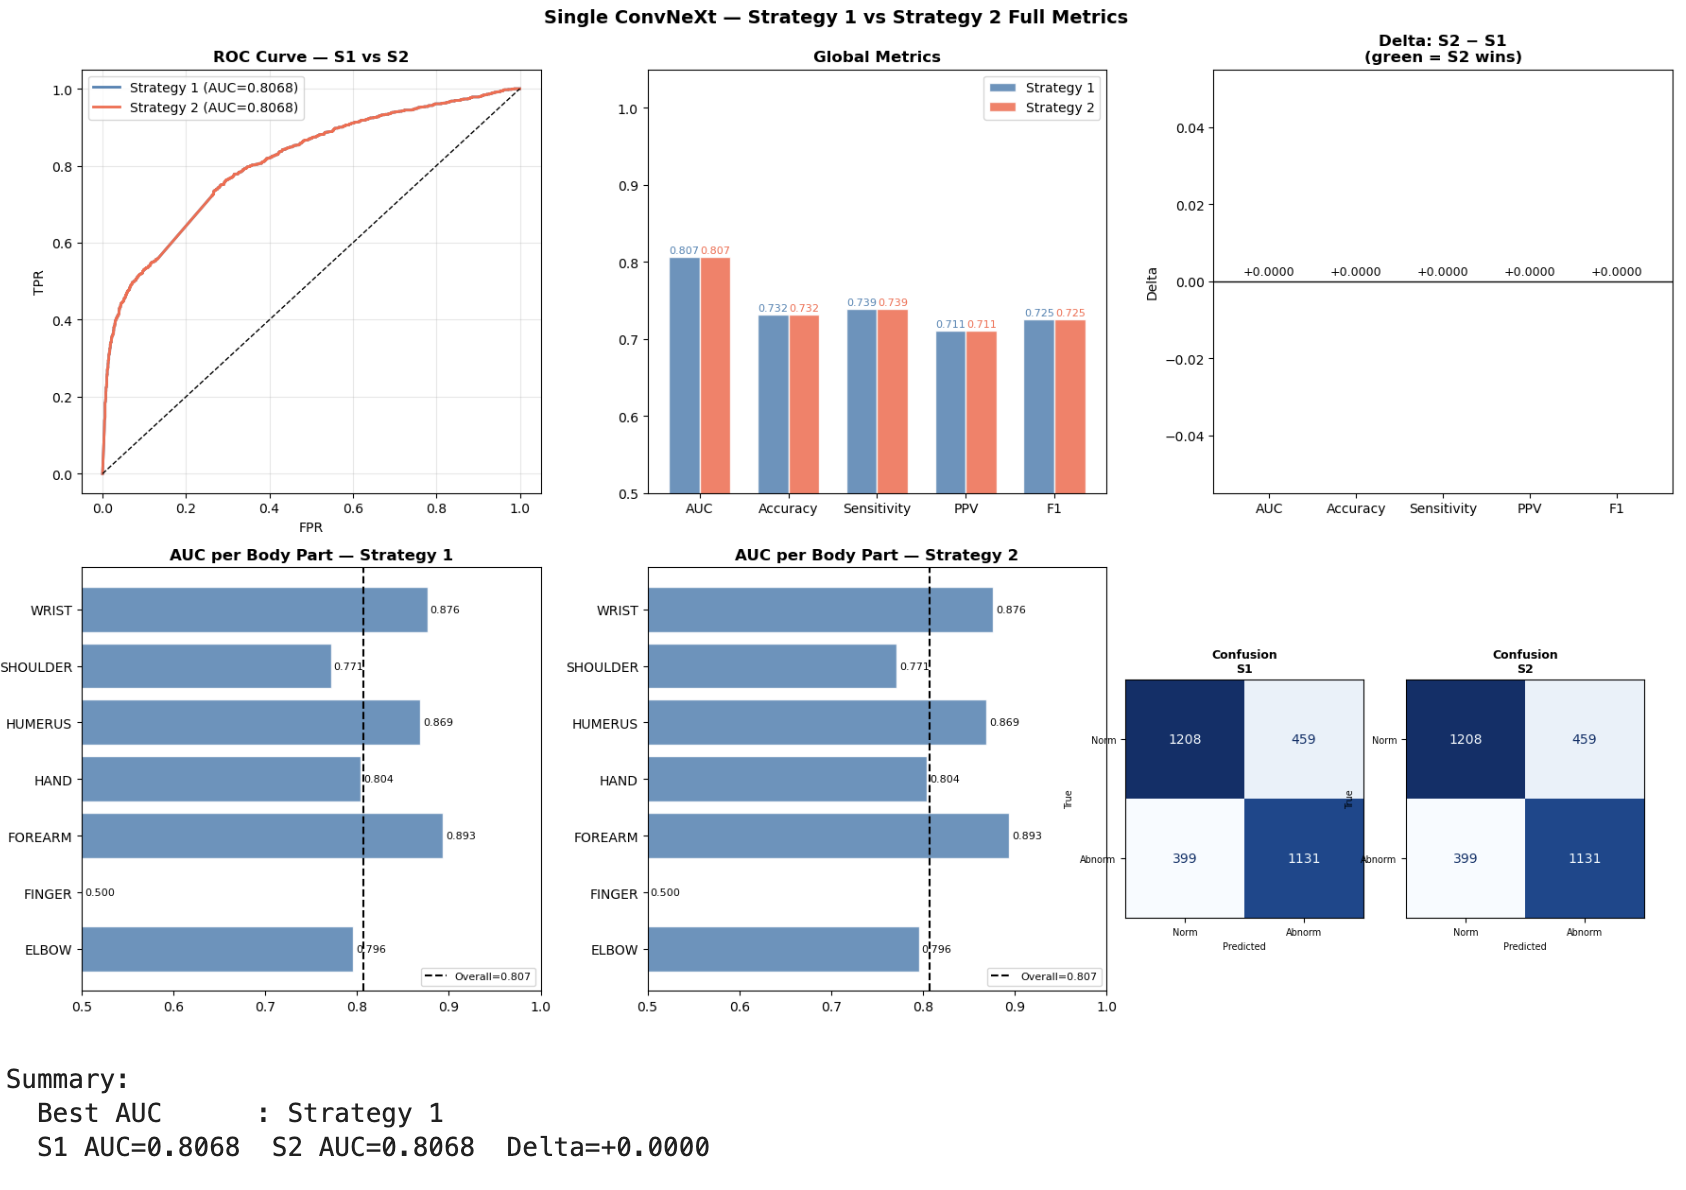
\includegraphics[width=\textwidth]{convnext_single_metrics.png}
    \caption{Model performance metrics across architectures.}
    \label{fig:metrics}
\end{figure*} 

\begin{figure*}[htbp]
    \centering
    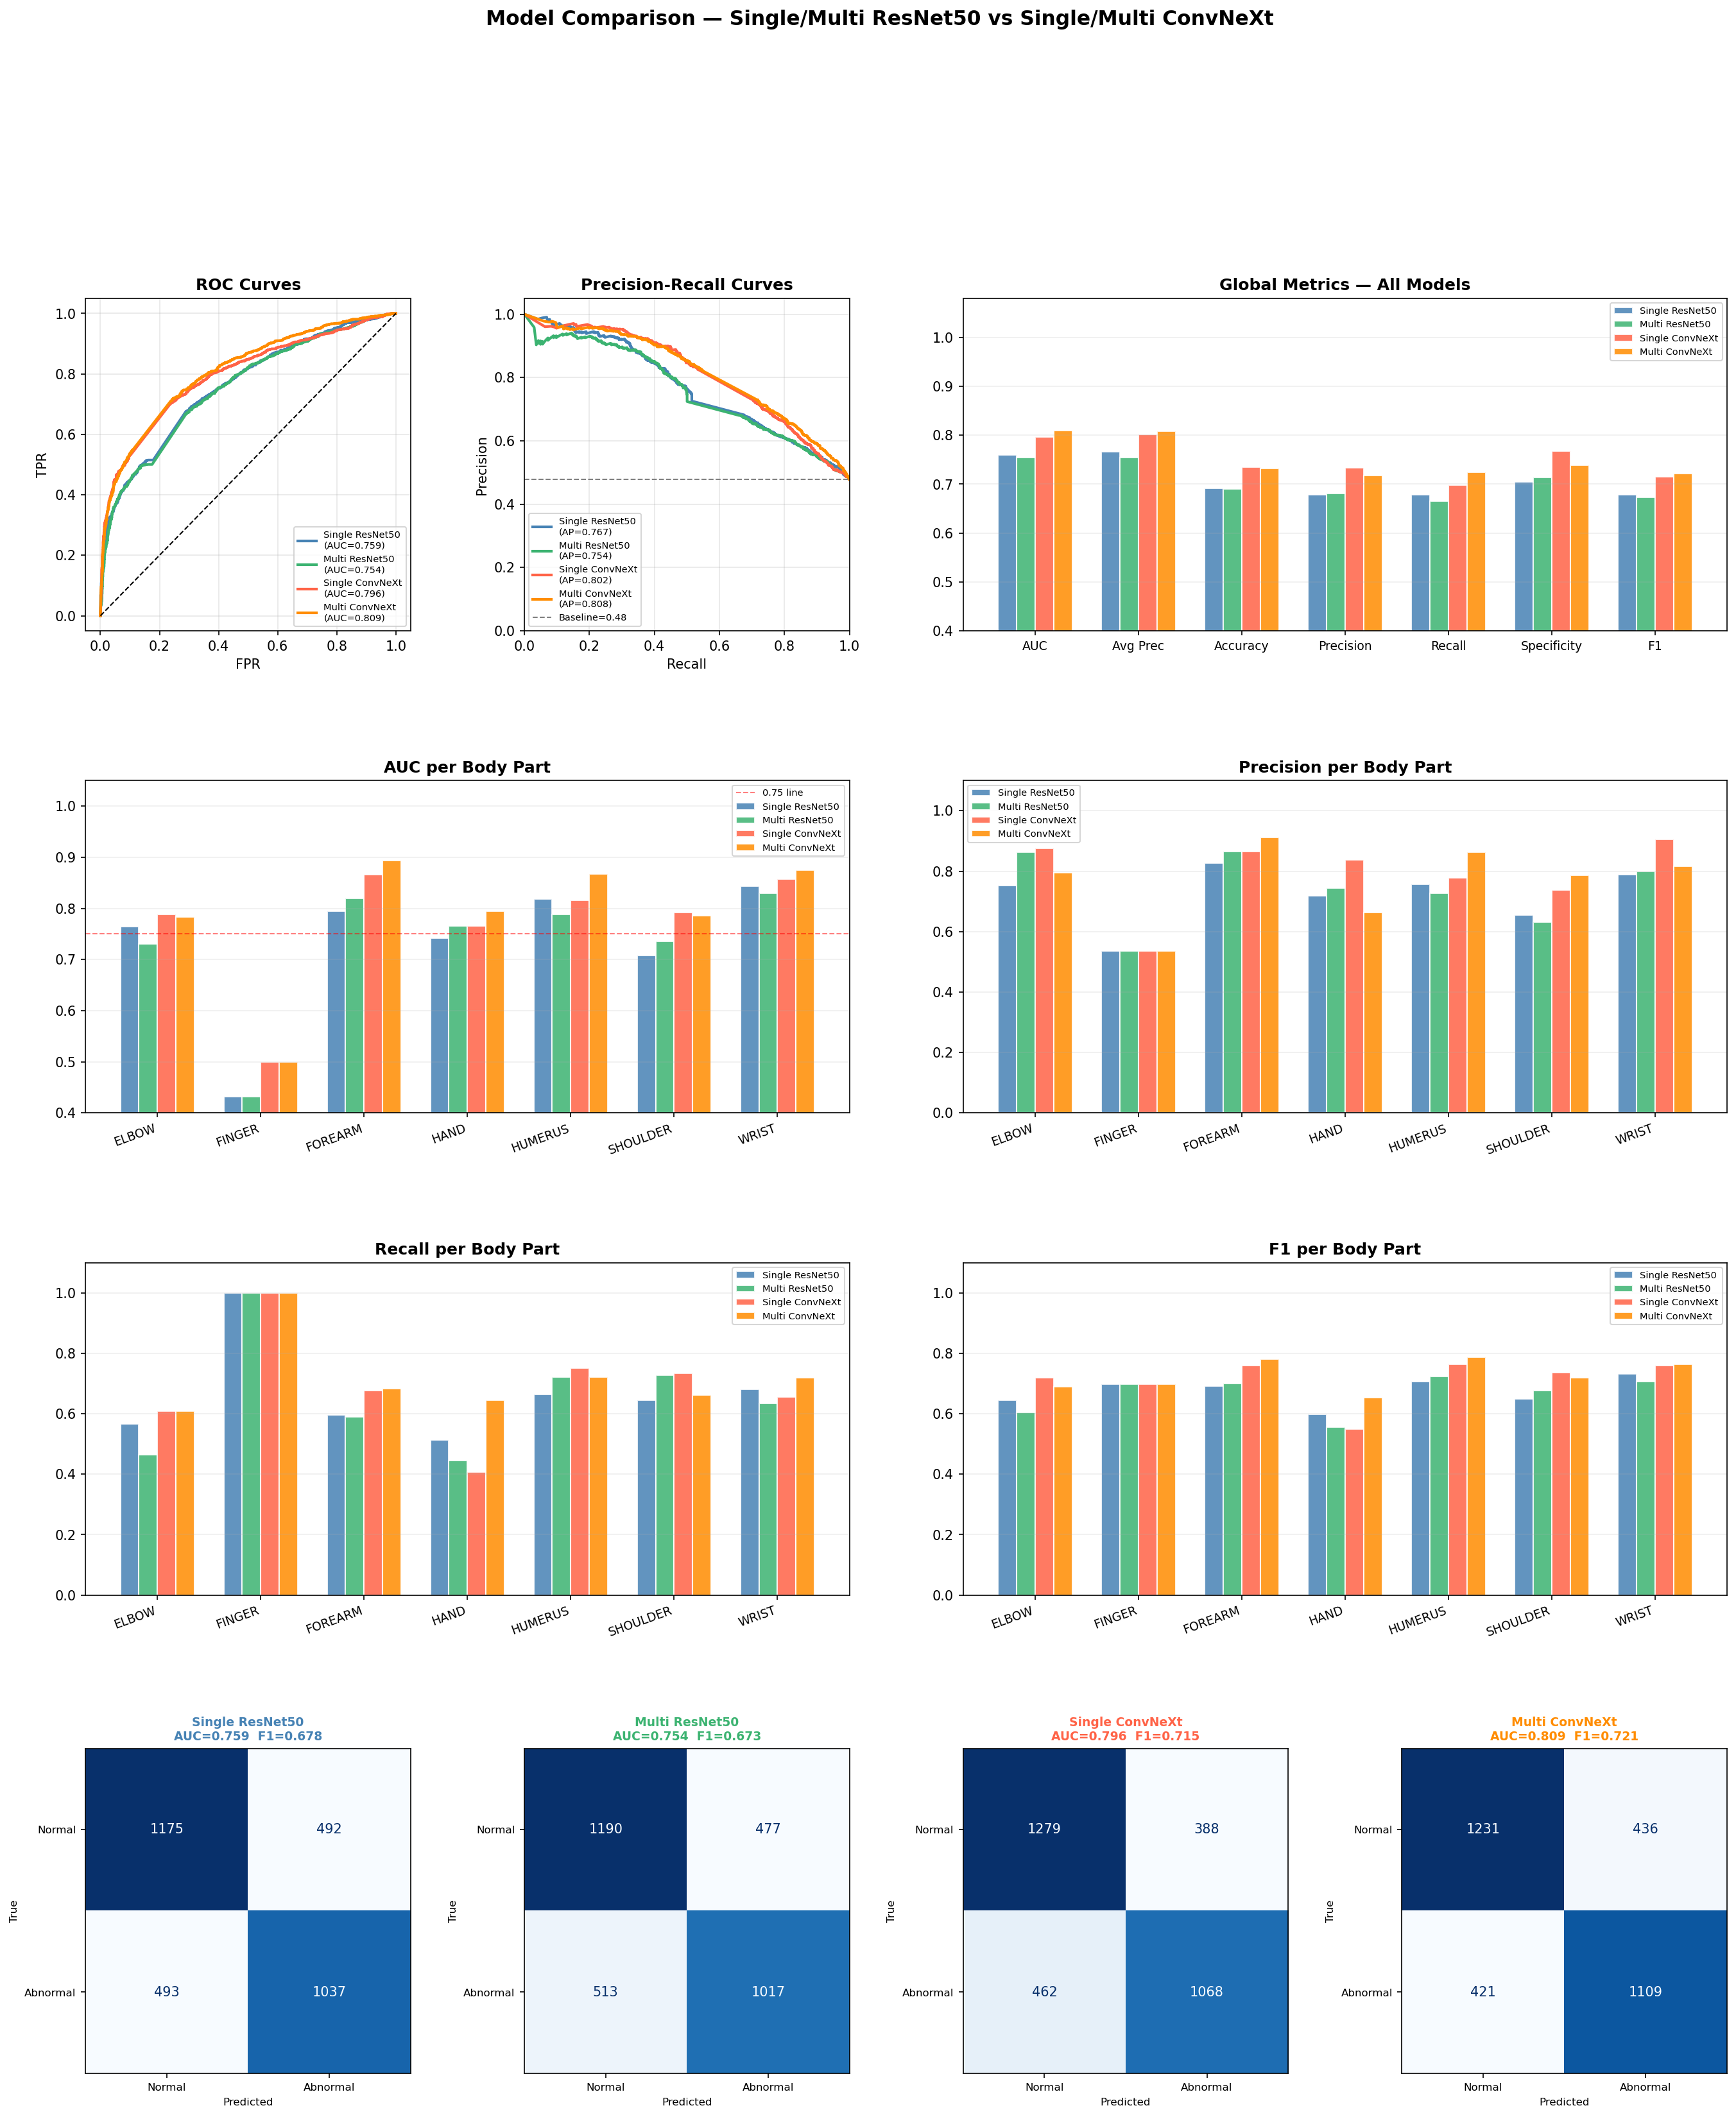
\includegraphics[width=\textwidth]{model_comparison_full_metrics_s1.png}
    \caption{Model performance metrics for Strategy1 data set}
    \label{fig:metrics}
\end{figure*} 


\begin{figure}[htbp]
    \centering
    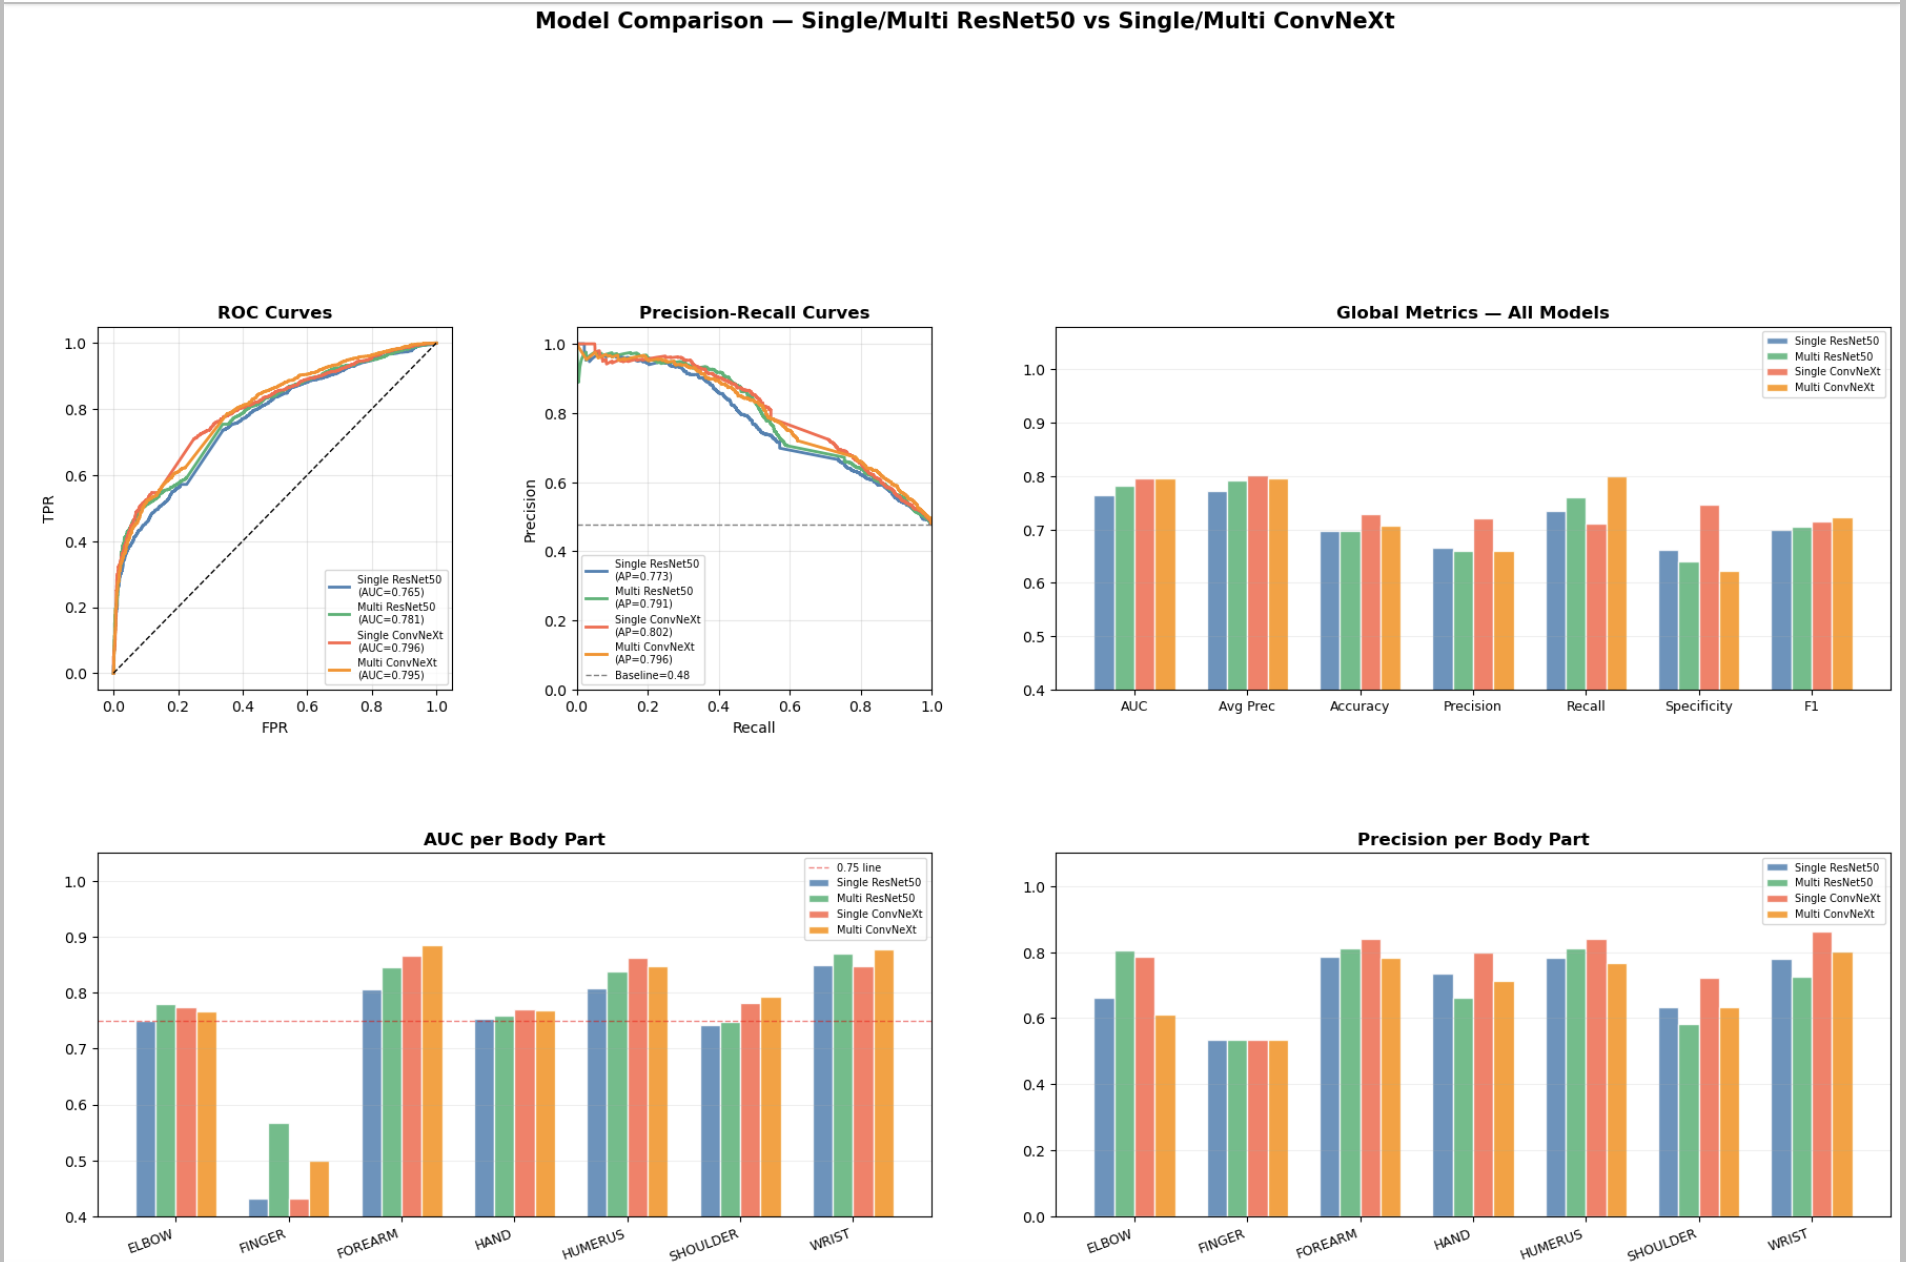
\includegraphics[width=0.95\linewidth]{ModelComparison_Strategy2_1.png}
    \caption{Model performance metrics for Strategy 2 data set}
    \label{3.1}
\end{figure}

\begin{figure}[htbp]
    \centering
    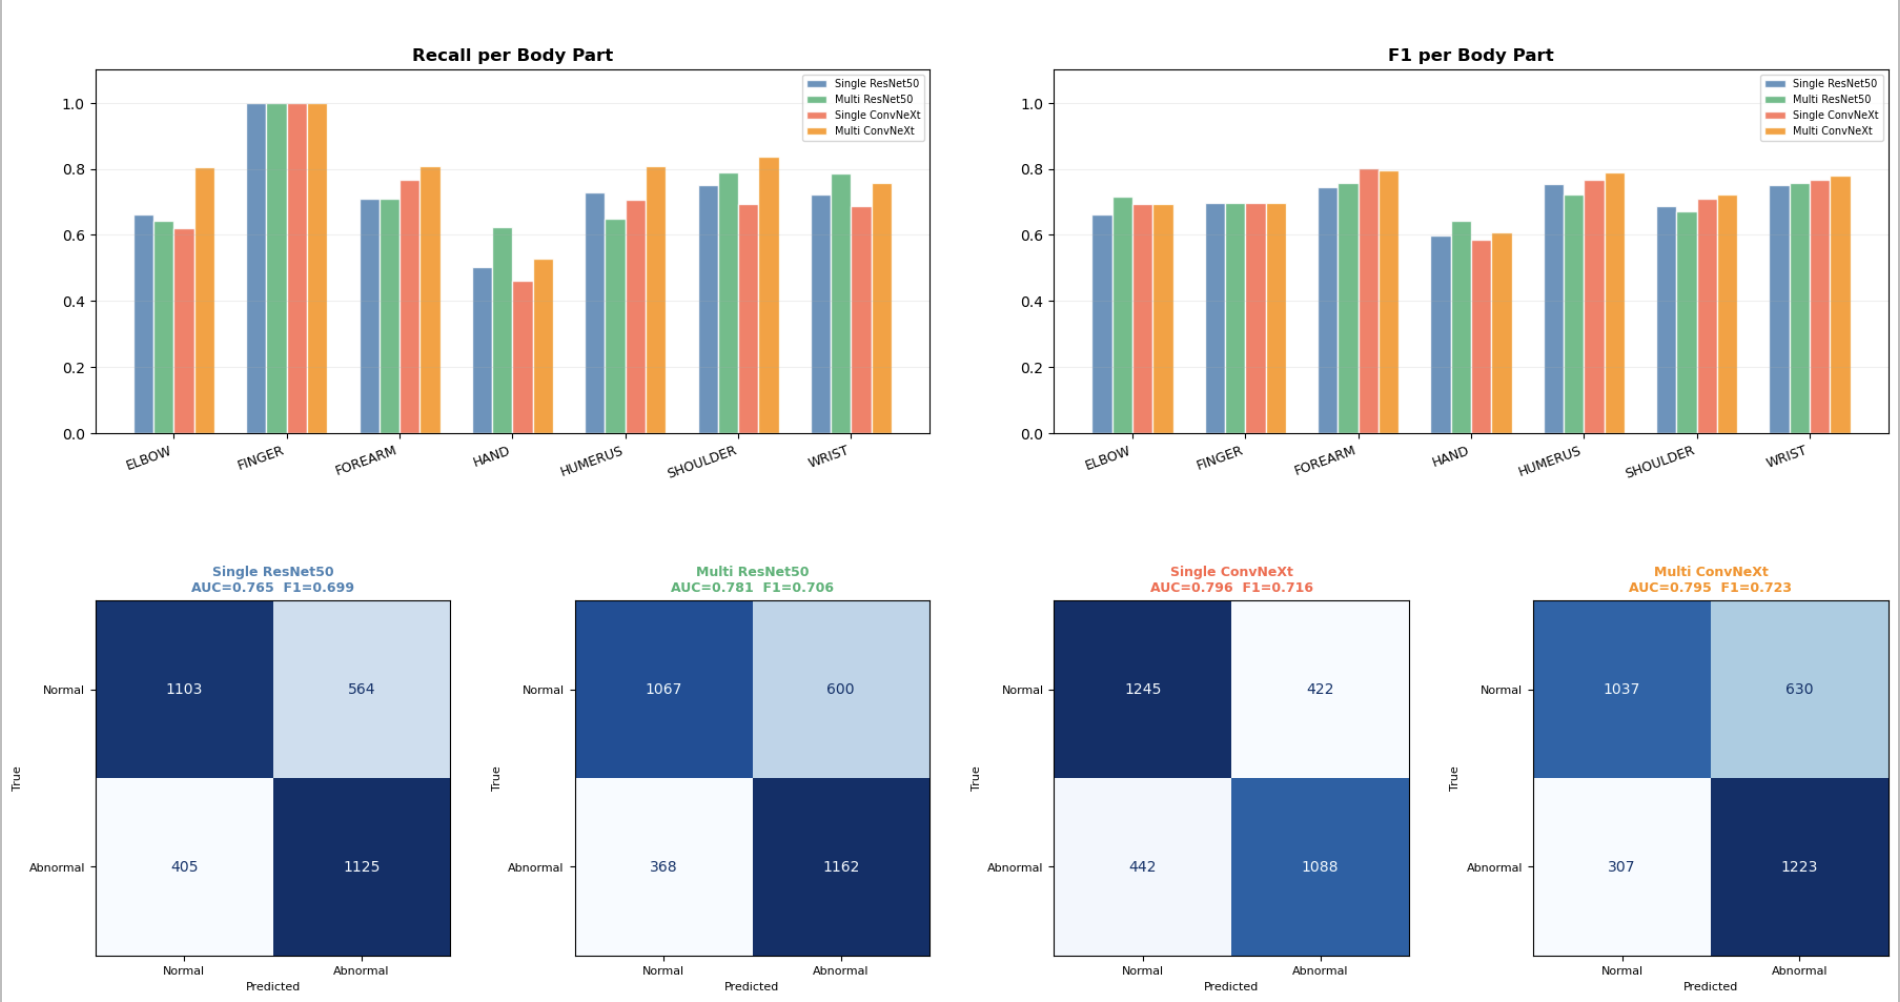
\includegraphics[width=0.95\linewidth]{ModelComparison_Strategy2_2.png}
    \caption{Model performance metrics for Strategy 2 data set}
    \label{fig:placeholder}
\end{figure}

\begin{table*}[t]
\centering
\caption{Summary of best-performing models across architectures and strategies.}
\label{tab:final_results}
\begin{tabular}{l l l c c c c c c c c}
\hline
Model & Task & Strategy & Epoch & Train Loss & Val Loss & AUC & Sens. & F1 & Acc. & Body Acc. \\
\hline
ConvNeXt & Single & S1 & 12 & 0.5499 & 1.2773 & 0.8178 & 0.7471 & 0.7365 & 0.7441 & -- \\
ConvNeXt & Multi  & S2 & 1  & 2.0803 & 2.1913 & 0.8182 & 0.7686 & 0.7403 & 0.7419 & 0.8026 \\
ResNet50 & Single & S1 & 3  & 0.5821 & 0.8507 & 0.7869 & 0.7595 & 0.7109 & 0.7044 & -- \\
ResNet50 & Multi  & S1 & 18 & 1.9469 & 1.5450 & 0.7850 & 0.7026 & 0.7038 & 0.7169 & 0.8033 \\
\hline
\end{tabular}
\end{table*}

\section{Preliminary Experiments \& Results}
\subsection{\textbf{Experiments and Hypotheses}}
To evaluate abnormality detection performance, both ResNet-50 and ConvNeXt architectures were assessed for abnormality detection accuracy with and without joint training on body part classification. The first hypothesis was that ConveNeXt would perform bettwe than ResNet50 for both classification tasks, due to its increased complexity. The second hypothesis was that abnormality detection accuracy would improve in a multitask model that simultaneously detects body part, making the model more sensitive to differences in bone structure. 

The multitask models performed both abnormality detection and body part classification. Body part classification accuracy was evaluated separately by body part for both the ResNet-50 and ConvNeXt architectures. The hypothesis was that body parts with more distinct bone structures, such as the hand, would be easier to detect than those with less intricate structures, such as the forearm. 

Multiple strategies were implemented in the training as well. In strategy 1 (S1), each study is treated separately and each image as its own observation. Strategy 2 (S2), only keeps one study by each patient (positive wins) and each image as its own observation. The hypothesis was that that Strategy 2 would have increased performance in both ConvNeXt and ResNet models, due to the uniform abnormality label from the study.

\subsection{\textbf{Results}}

\subsubsection{Confusion Matrix Metrics}
Across all 8 model-strategy combinations [Fig 2][Fig 3][Fig 4], the total validation set holds 1,667 normal and 1,530 abnormal images. Multi ConvNeXt S2 delivers the strongest clinical profile with the lowest false negatives at 307 — meaning it misses the fewest real fractures of any combination tested. However it carries the highest false positive count at 630, flagging the most healthy cases incorrectly.
Multi ConvNeXt S1 presents the opposite tradeoff — only 436 false positives but 421 false negatives, making it the most precise but less sensitive option.
ResNet50 variants consistently underperform both ConvNeXt models. Multi ResNet50 S1 is the weakest overall with 513 false negatives — the highest missed fracture count across all 8 combinations, making it the least clinically safe option tested.
The consistent pattern: ConvNeXt backbones reduce false negatives by 100–200 cases versus ResNet50 equivalents, and Strategy 2 training reduces false negatives further at the cost of more false positives.

\subsubsection{AUC and ROC Analysis}
Area under the ROC curve (AUC) was used as the primary threshold-independent metric to compare classification ability across training strategies. Among the single-task models, Strategy 1 (S1) consistently produced stronger AUC values than Strategy 2 (S2). For the ConvNeXt architectures, S1 achieved an AUC of 0.8178 compared to 0.8099 for S2. For the ResNet50 model, S1 achieved an AUC of 0.7869 compared to 0.7829 for S2.

In the multi-task setting, results varied by architecture type. ConvNeXt achieved the highest overall AUC of 0.8182 with S2 compared to 0.8162 for S1. In contrast, ResNet50 performed better under Strategy 1, achieving an AUC of 0.7850 with S1 compared to 0.7806 for S2. 

Looking more broadly at the trends in AUC across the four classification models, we see ConvNeXt showed stronger ROC performance than ResNet50 in both single-task and multi-task settings, suggesting that it learned more discriminative features for abnormality detection. 


However, we did not see significant improvement in AUC for abnormality detection from single task to multi task models of the same architecture type. Multi-task detection slightly improved scores for the ConvNeXt arhtectures, however, reduced the AUC for ResNet50 based models. This indicates that the addition of body part classification may not improve abnormality detection, as originally hypothesized. 

\subsubsection{Accuracy and F1 Score}
Model performance was evaluated using Accuracy and F1-score, with the latter serving as a robust metric for imbalanced medical data by balancing precision and recall. In single-task experiments, the ConvNeXt architecture consistently outperformed ResNet-50, achieving a peak F1-score of 0.7365. While single-task models generally maintained higher raw accuracy, their performance proved sensitive to data handling strategies, often dipping when the training signal was altered.

In contrast, multitask models demonstrated a more nuanced and resilient performance profile. Although shifting to a multitask configuration caused a slight decrease in overall accuracy, it significantly enhanced the model's ability to generalize. Notably, the multitask ConvNeXt surpassed all single-task configurations with a top F1-score of 0.7403. These results suggest that while single-task models may excel in isolated benchmarks, multitask architectures leverage complex training signals more effectively, ultimately providing a more balanced and superior evaluation for clinical applications.

\subsection{\textbf{Overall Performance}}
We implemented four classification models: single- and multi-task versions of ResNet and ConvNeXt. Model performance was evaluated using AUC, F1 score, accuracy, sensitivity, and training/validation loss. We tested four main hypotheses: (1) ConvNeXt would outperform ResNet, (2) multi-task classification would improve abnormality detection accuracy, (3) training strategy 2 would outperform strategy 1, and (4) body parts with more unique structures would achieve higher classification accuracy.

Looking at Figure 1, we can see that ConvNext, in general, achieved higher classification metrics across the board in comparison to ResNet50 architectures. Interestingly, multi-task classification did not improve abnormality detection for either ConvNeXt or ResNet models. Optimal training strategy was found to be architecture dependent, with strategy 1 performing between for both ResNet models, and strategy 2 performing better only for the multi-task ConvNeXt model. This may indicate that as model complexity increases, a preference for more uniform classifications like the ones present in strategy 2, is preferred. Lastly, we saw across models that body parts of the wrist, shoulder, and humerus had the highest AUC. This contradicts our hypothesis that body parts with more unique structures, such as the hand or shoulder, would have higher classification metrics. Instead, more general smooth structure, those that are single rectangular bones such as the forearm and humerus had the highest AUC across models. 

\section{Next Steps}
Looking ahead to our next milestone, we have identified several areas of focus for the coming weeks. Our first priority is selecting a single training strategy for our models; we are currently leaning toward strategy 1 but continue to weigh the trade-offs between both approaches. Second, we aim to understand why earlier epochs yield better accuracy for certain models. Metrics were initially selected based on AUC at optimal points, which favored earlier epochs for some models; in the next phase, we plan to standardize epoch selection and redo metric comparisons. Additional goals include improving visualizations for metric comparisons and advancing the implementation and testing of FracAtlas across all four models to better assess generalizability. 


\section{Declaration on Generative AI}
The authors used ChatGPT and Grammarly to check grammar and spelling as well as reword author-written work. After using these tools, the authors reviewed and edited the final text, used in this document. 

\section{Individual Contributions}

Jasmine Waller: Contributed to building the ConvNeXt model architecture, training, and model evaluation, as well as helped with writing the report.

Kristina Quintana: Contributed to preparing the dataset by providing to code for resplitting the data and creating the two training sets. Also contributed analyzing the metrics and adding to the writing of the report

Claire Sullivan: Contributed to the building of the ResNet50 model architecture, training, and evaluation, as well as helped with the writing of the report. 

Srivatsa Balasubramanyam: Contributed to the EDA and buidling the data loaders. Also worked on overall execution of the model in Rivanna and metrics for model comparison of 8 models across 2 strategy datasets

\bibliographystyle{IEEEtran}  
\bibliography{refs}         
\bibliographystyle{unsrt}

\end{document}
